\section{Les figures}


% exemple d'une figure
% - placement de la figure dans les [] : h, t, b, H, !h ...
\begin{figure}[H]
	\centering
	\caption{Légende figure}
	\label{fig:label_figure}
	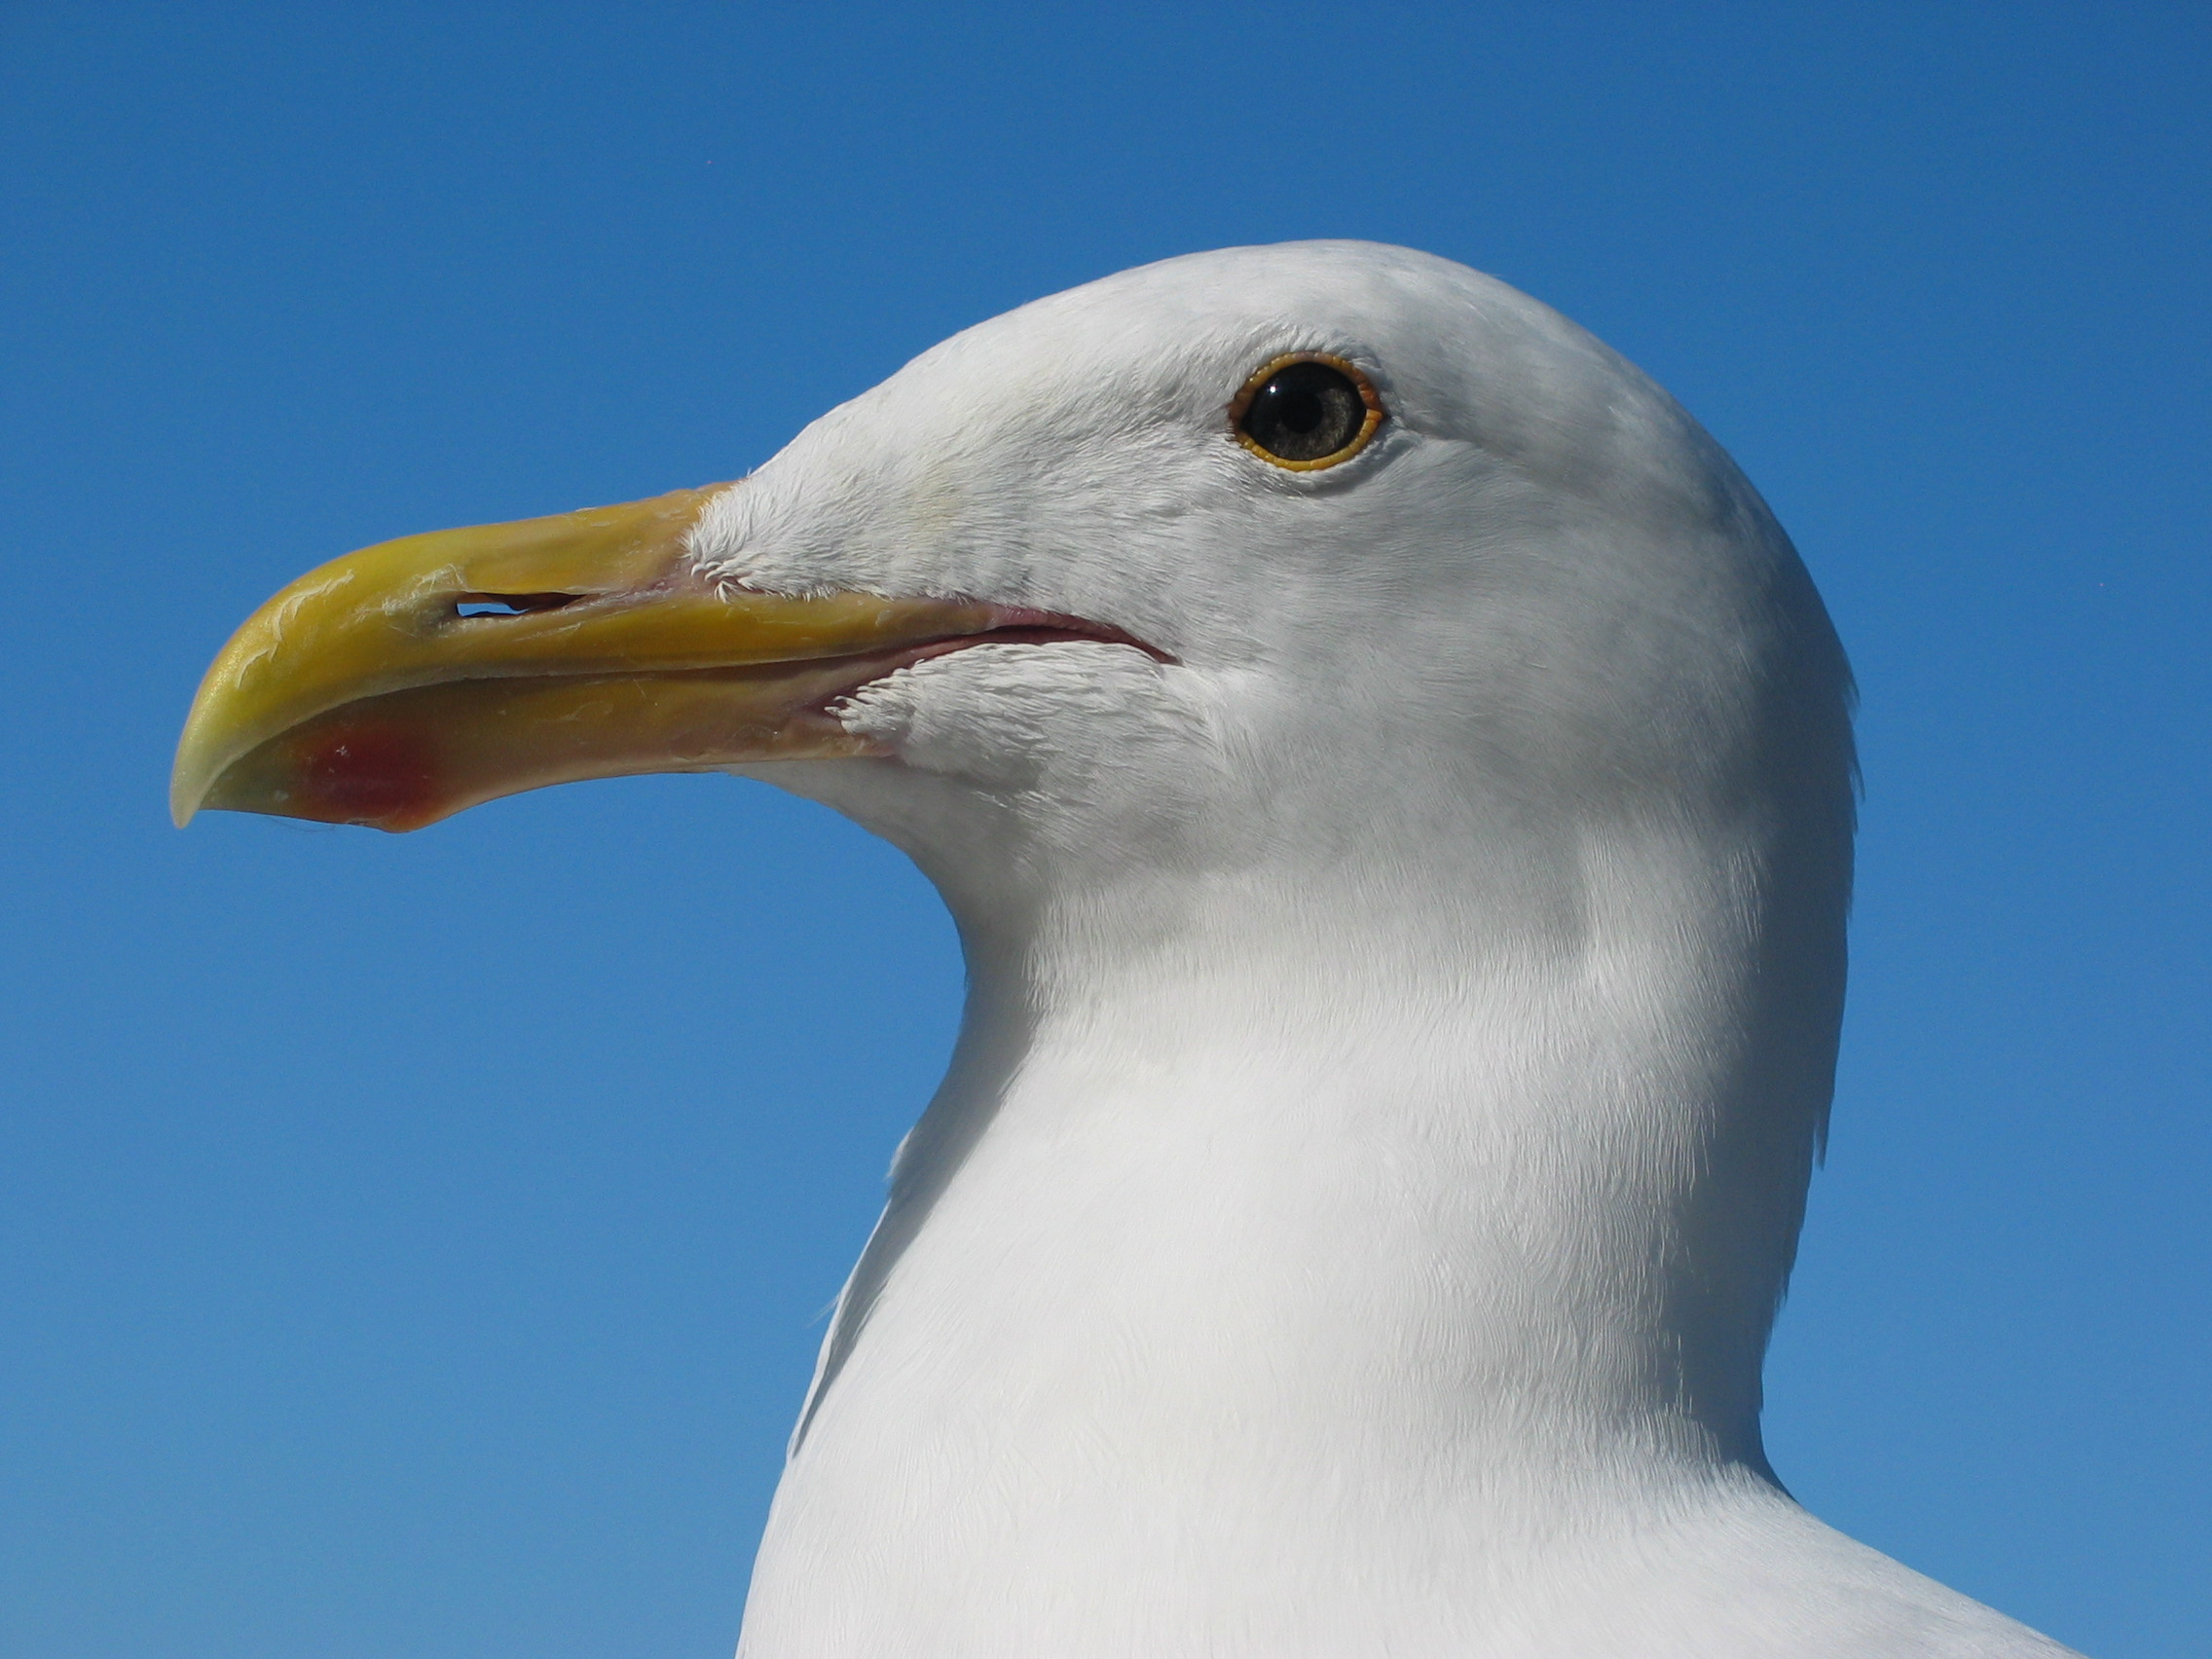
\includegraphics[width=0.5\textwidth]{images/gull}	
\end{figure}


% plusieurs figures côtes à côtes 
% voir : http://blog.pengyifan.com/the-best-way-to-place-figures-side-by-side-in-latex/
\begin{figure}
	\centering
	
  	\begin{subfigure}[b]{0.4\textwidth}
    		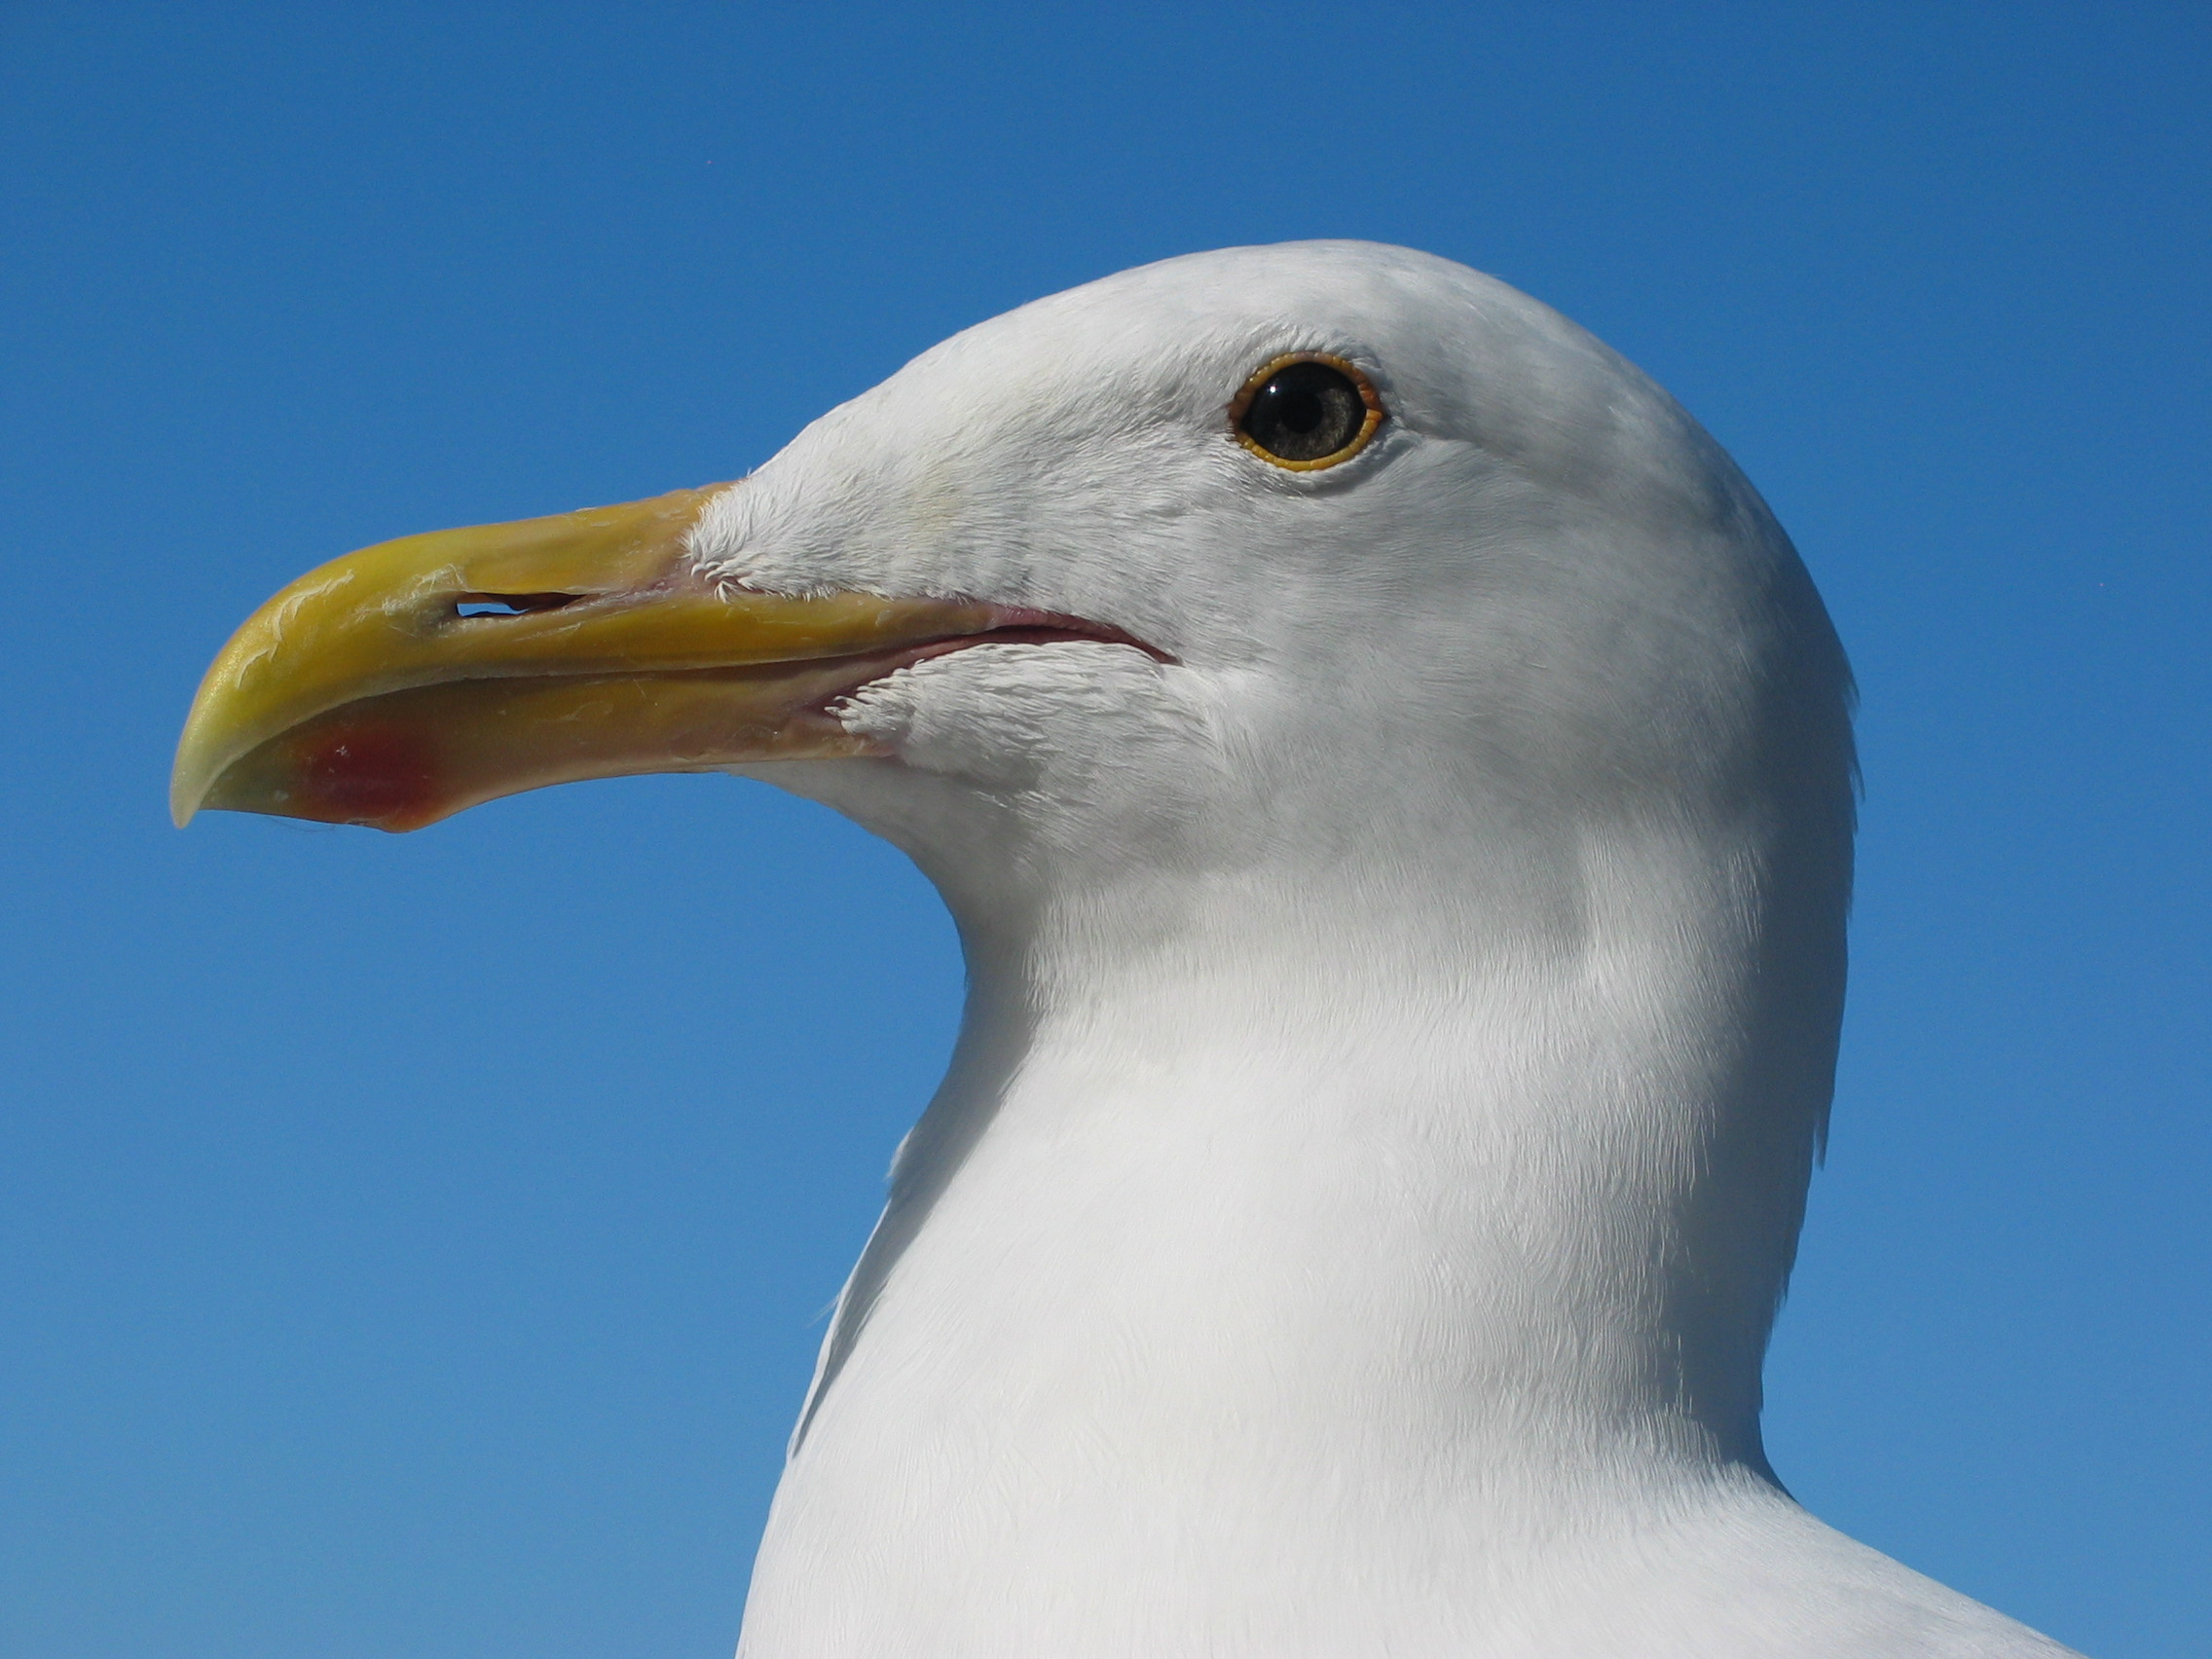
\includegraphics[width=\textwidth]{images/gull}
    		\caption{Picture 1}
    		\label{fig:1}
  	\end{subfigure}
  	\begin{subfigure}[b]{0.4\textwidth}
    		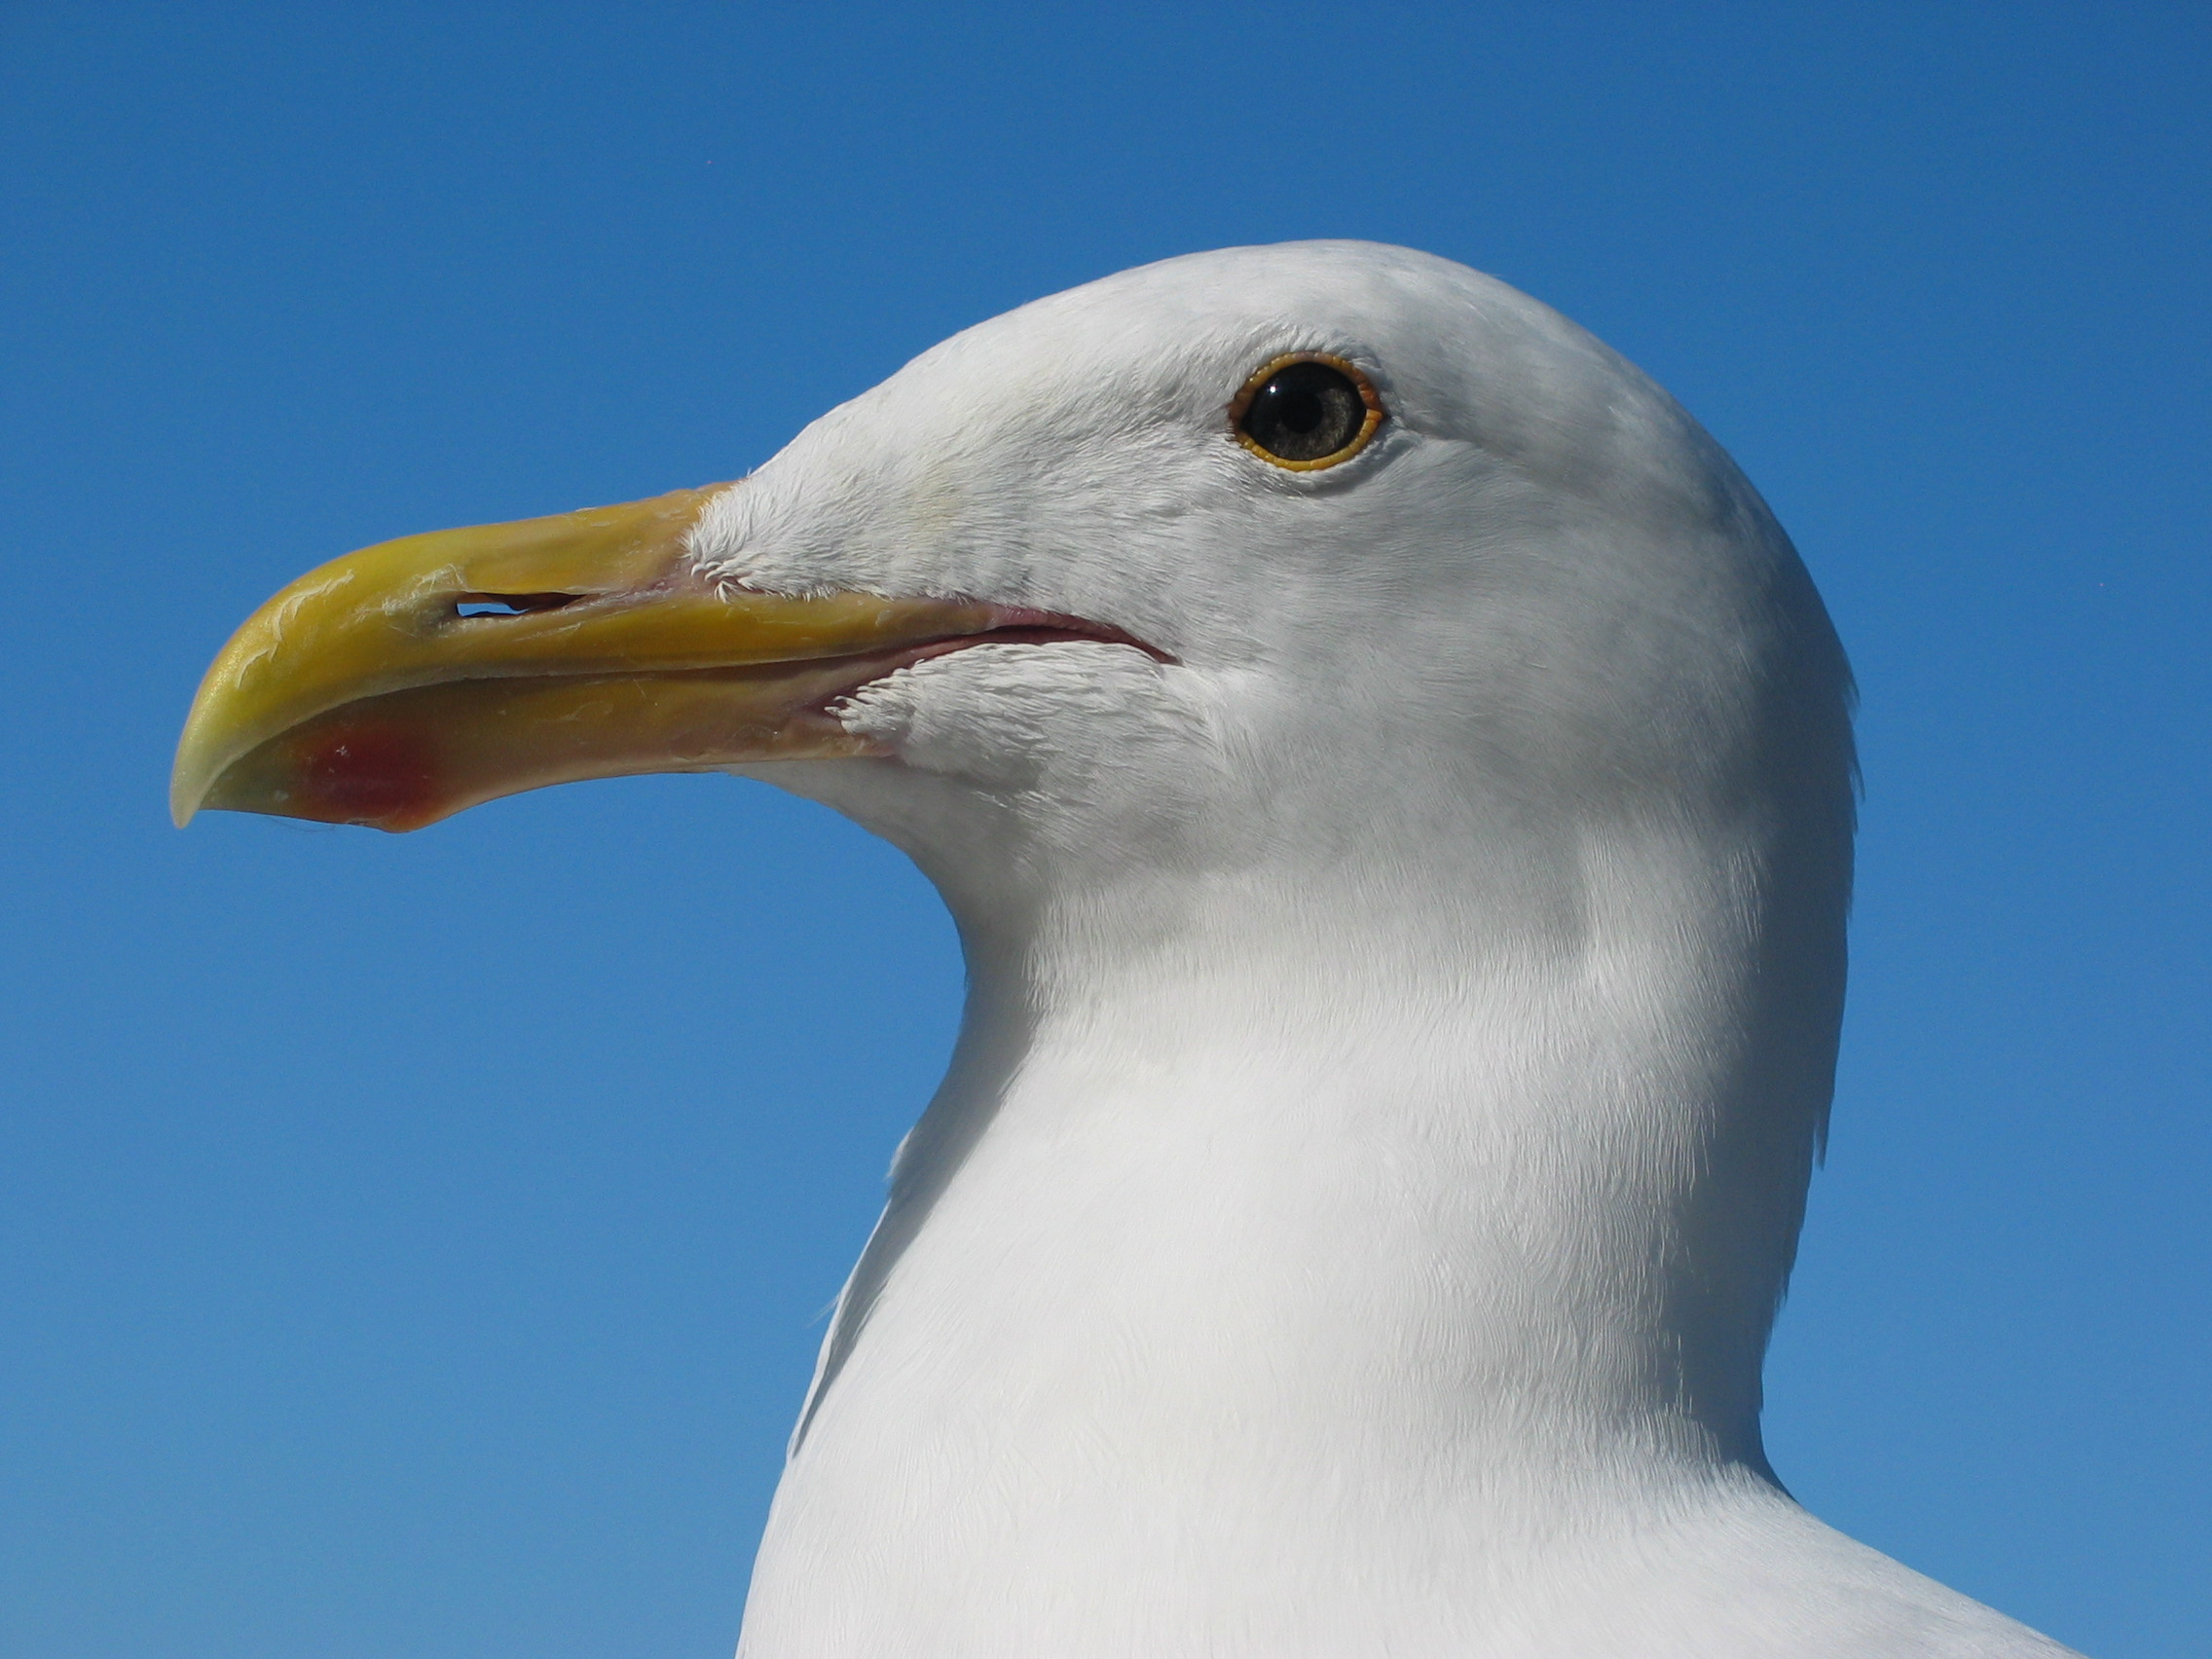
\includegraphics[width=\textwidth]{images/gull}
    		\caption{Picture 2}
    		\label{fig:2}
  	\end{subfigure}
	
	\caption{global}
\end{figure}










}
%%%%%%%%%%%%%%%%%%%%%%%%%%%%%%%%%%%%%%%%%%%%

\begin{frame}{Tests de comparaison}
  \begin{figure}
      %\centering
      
        \begin{subfigure}[b]{1\textwidth}
            \parbox[b]{.5\linewidth}{
            \includegraphics[height=0.2\textwidth]{images/comparaison/vod_ClapprEB/distribution_of_bandwidth}
            }
            \parbox[b]{.4\linewidth}{
                \caption{Clappr}
            }
        \end{subfigure}
        
        \begin{subfigure}[b]{1\textwidth}
            \parbox[b]{.5\linewidth}{
                \includegraphics[height=0.2\textwidth]{images/comparaison/vod_DashEB/distribution_of_bandwidth}
            }
            \parbox[b]{.4\linewidth}{
                \caption{DashEB 1.0}
            }
        \end{subfigure}
        
        \begin{subfigure}[b]{1\textwidth}
            \parbox[b]{.5\linewidth}{
                \includegraphics[height=0.2\textwidth]{images/comparaison/vod_DashEB2/distribution_of_bandwidth}
            }
            \parbox[b]{.4\linewidth}{
                \caption{DashEB 2.0}
            }
        \end{subfigure}
      
      \caption{diffusion VOD}
    \end{figure}
\end{frame}




